\documentclass{article}

% Top margin, right margin, left margin, bottom margin, footnote skip
\usepackage[utf8]{inputenc}
\usepackage{biblatex}
\addbibresource{./references.bib}
% linktocpage shall be added to snippets.
\usepackage{hyperref,theoremref}
\hypersetup{
	colorlinks, 
	linkcolor={red!40!black}, 
	citecolor={blue!50!black},
	urlcolor={blue!80!black},
	linktocpage % Link table of content to the page instead of the title
}

\usepackage{blindtext}
\usepackage{titlesec}
\usepackage{amsthm}
\usepackage{thmtools}
\usepackage{amsmath}
\usepackage{amssymb}
\usepackage{graphicx}
\usepackage{titlesec}
\usepackage{xcolor}
\usepackage{multicol}
\usepackage{hyperref}
\usepackage{import}
\usepackage{libertinus}           % Load the Libertinus font
\usepackage{mathbbol}
\usepackage{bm}
\usepackage{mathrsfs}

\usepackage{tikz}
\usepackage{tikz-cd}
\usetikzlibrary{arrows.meta, positioning, calc, arrows}
% \usepackage{calrsfs}


\newtheorem{theorem}{Theorem}[section]
\newtheorem{lemma}[theorem]{Lemma}
\newtheorem{corollary}{Corollarium}[section]
\newtheorem{proposition}{Proposition}[theorem]
\theoremstyle{definition}
\newtheorem{definition}{Definition}[section]

\theoremstyle{definition}
\newtheorem{axiom}{Axioma}[section]

\theoremstyle{remark}
\newtheorem{remark}{Remark}[section]
\newtheorem{hypothesis}{Coniectura}[section]
\newtheorem{example}{Exampli Gratia}[section]
% Proof Environments
\newcommand{\thm}[2]{\begin{theorem}[#1]{}#2\end{theorem}}

% \renewenvironment{proof}{{\bfseries\emph{Demonstratio.}}}{\qed}
\renewcommand\qedsymbol{Q.E.D.}

\newcommand{\D}{\bm{\Delta}}
\renewcommand{\S}{\textbf{Set}}
\newcommand{\sS}{\textbf{sSet}}
\newcommand{\op}{^{\text{op}}}
\newcommand{\N}{\mathbb{N}}
\renewcommand{\L}{\Lambda}
\newcommand{\C}{\mathcal{C}}
\newcommand{\F}{\text{Fun}}

\let\H\relax
\DeclareMathOperator{\H}{\text{Hom}}

\renewcommand{\emph}{\textbf}


\title{$\infty$-Category and Simplicial Sets}
\author{Candidate Number: 1099144} 
\date{\today}

\begin{document}

\maketitle

\tableofcontents

\section{Simplex Category and Simplicial Sets}

\subsection{Definition of Simplical Sets}

The goal of this mini-project to to define $\infty$-categories via simplicial sets. 
The definition of simplicial sets is based on the \emph{simplex category}, $\D$.

\begin{definition}[Simplex Category \cite{lurie}]
	The \emph{simplex category}, denoted as $\D$, is defined as
	\begin{enumerate}
		\item Its objects linearly ordered finite sets $[n] = \{0 < 1 < \cdots < n\}$ for all $n \geq 0$.
	\item Its morphisms are given by order-preserving maps.
	\end{enumerate}
	Simplex category is also known as the category of combinatorial simplices
\end{definition}

It is clear that $\D$ is equivalent to the category of all finite non-empty totally ordered sets with order-preserving maps. 

For each $n, j \in \N, 0\leq j \leq n$, define \emph{face} and \emph{degenerate} maps repectively as $\D$, $d^{j,n}: [n - 1] \to [n]$ and $s^{j, n}: [n + 1] \to [n]$ given by
\begin{equation}
	d^{j, n}(i) = \begin{cases}
		i & i < j \\
		i + 1 & i \geq j
	\end{cases}, \quad
	s^{j,n}(i) = \begin{cases}
		i & i \leq j \\
		i - 1 & i > j
	\end{cases}.
\end{equation}

Concretely, the face map $d^{j, n}$ is the only injective and order-preserving maps from $[n - 1]$ to $[n]$ that misses $j \in [n]$, and the degenerate map $s^{j, n}$ is the only surjective and order-preserving map from $[n + 1]$ to $[n]$ that hits $j \in [n]$ twice.

Since the domain and codomain of the face and degenerate maps will always be clear from the context, we will drop the superscripts and denote them as $d^j$ and $s^j$.

Let $i < j$. 
The composition of face maps $d^jd^i$ is the unique injective and order-preserving map from $[n - 2]$ to $[n]$ that misses both $i$ and $j \in [n]$. 
A moment of thought shows that this map is the same as $d^id^{j - 1}$.
There are similar relations for the compositions of degenerate maps and mixed compositions of face and degenerate maps. 
All of the identities are listed below.

% TODO: check the middle case
\begin{align}
	d^jd^i &= d^id^{j - 1}, \quad i < j \label{sim1} \\
	s^js^i &= s^is^{j + 1}, \quad i \leq j  \label{sim2} \\
	s^j d^i &= \begin{cases}
		d^i s^{j - 1} & j < i \\
		\text{id} & j = i, i + 1 \\
		d^{i - 1} s^j & j > i + 1
	\end{cases} \label{sim3}
\end{align}

It can be shown that all morphisms in $\D$ can be generated by compositions of face and degenerate maps.

We are now ready to define simplicial sets.

\begin{definition}[Simplicial Set \cite{lurie}]
	A \emph{simplicial set} is presheaf on $\D$, i.e.,
	a functor $X: \D\op \to \S$. 
	We will denote the category of simplicial sets as $\sS$.
\end{definition}

Let $X$ be a simplicial set.
Define $X_n := X([n])$.
We shall define the face map $d_j: X_n \rightarrow X_{n-1}$ as the map induced by the face map on $\D$, $d^j: [n - 1] \to [n]$. 
That is $d_j = Xd^j$. 
Similarly, denote $s_j: X_n \to X_{n + 1}$ the map induced by the degenerate map $s^j: [n + 1] \to [n]$, i.e., $s_j = Xs^j$.
Since $X$ is contravariant, $d_j$ and $s_j$ will satify the following identities, reversing the order of composition compared to \eqref{sim1}, \eqref{sim2}, and \eqref{sim3}. 

\begin{align}
	d_i d_j &= d_{j - 1} d_i, \quad i < j \label{simp1} \\
	d_i s_j &= \begin{cases}
		s_{j - 1} d_{i} & j < i \\
		\text{id} & j = i, i + 1 \\
		s_{j} d_{i - 1} & j > i + 1
	\end{cases} \label{simp3} \\
	s_i s_j &= s_{j + 1} s_i, \quad i \leq j  \label{simp2} 
\end{align}

Since $d^j$ and $s^j$ generates all morphisms in $\D$, the morphisms $d_j$ and $s_j$ will generate all relevant morphisms in $\S$ relevant to $X$ (Recall $X \in [\D\op, \S]$). 
This gives a crucial observation. 

\begin{remark}\label{sim-set-data}
The data given by a simplicial set $X$ is equivalent to the data of a sequence of sets $\{X_n\}_{n \geq 0}$ together with face and degenerate maps $d_j: X_n \to X_{n - 1}$ and $s_j: X_n \to X_{n + 1}$ satisfying the identities \eqref{simp1}, \eqref{simp2}, and \eqref{simp3}.
\end{remark}

\subsection{Horn and Simplices}

The first intuitive example of simplicial sets are the standard simplices, which are the Yoneda embeddings of the objects in $\D$.

\begin{definition}[Standard n-Simplex \cite{lurie}]
	For each $n \geq 0$, the \emph{standard n-simplex}, denoted as $\Delta^n$, is defined as the contravairant functor
	\begin{equation*}
		\Delta^n := \H_{\D}(-, [n]): \D\op \to \S.
	\end{equation*}
\end{definition}

The zero-simplex is called vertices, the one-simplex edges, and the two-simplex triangles.
The reason for such nomenclature is that, the geometric realisation of zero-simplices, denoted as $|\Delta^0|$, is a point, while the geometric realisations of one- and two-simplices is a line segment and a triangle respectively.

$$
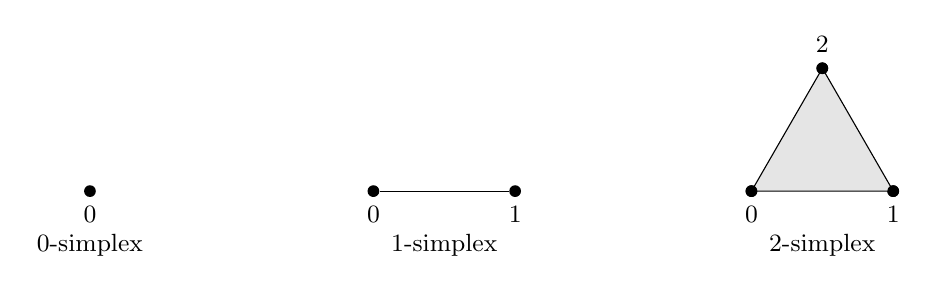
\begin{tikzpicture}[scale=1.2, every node/.style={font=\small}]

% ---- 0-simplex ----
\node[circle, fill=black, inner sep=1.5pt] (v0) at (0,0) {};
\node[below=2pt] at (v0) {$0$};
\node[below=12pt] at (0,0) {0-simplex};

% ---- 1-simplex ----
\node[circle, fill=black, inner sep=1.5pt] (v1a) at (3,0) {};
\node[circle, fill=black, inner sep=1.5pt] (v1b) at (4.5,0) {};

\draw (v1a) -- (v1b);

\node[below=2pt] at (v1a) {$0$};
\node[below=2pt] at (v1b) {$1$};

\node[below=12pt] at (3.75,0) {1-simplex};

% ---- 2-simplex ----
\node[circle, fill=black, inner sep=1.5pt] (v2a) at (7,0) {};
\node[circle, fill=black, inner sep=1.5pt] (v2b) at (8.5,0) {};
\node[circle, fill=black, inner sep=1.5pt] (v2c) at (7.75,1.3) {};

% \filldraw[fill=gray!20, draw=black] 
%   (v2a.center) -- (v2b.center) -- (v2c.center) -- cycle;
\draw[fill=gray!20] (v2a.center) -- (v2b.center) -- (v2c.center) -- cycle;

\node[circle, fill=black, inner sep=1.5pt] at (v2a.center) {};
\node[circle, fill=black, inner sep=1.5pt] at (v2b.center) {};
\node[circle, fill=black, inner sep=1.5pt] at (v2c.center) {};

\node[below=2pt] at (v2a) {$0$};
\node[below=2pt] at (v2b) {$1$};
\node[above=2pt] at (v2c) {$2$};

\node[below=12pt] at (7.75,0) {2-simplex};

\end{tikzpicture}
$$

Another important class of simplicial sets are horns, which can be thought of as simplices with one face missing.

\begin{definition}[Horn \cite{lurie}]
	For each $n \geq 1$ and $0 \leq i \leq n$, the \emph{$i$-th horn}, denoted as $\L^n_i$, is the simplicial defined as
	\begin{enumerate}
		\item $\L^n_i([m]) = \{f \in \H_{\D}([m], [n]) : [n] \smallsetminus \{i\} \not\subseteq f([m])\}$. 
			In other words, $\L^n_i ([m])$ is the set of all order-preserving maps from $[m]$ to $[n]$ that miss at least one element in $[n] \smallsetminus \{i\}$.
			For the sake of simplicity, we will denote $\L^n_i [m] := \L^n_i ([m])$.
		\item For a map $s \in \H_{\D} ([m], [k])$, the corresponding map $\L^n_i(s): \L^n_i[k] \rightarrow \L^n_i[m]$ are its pullback (see figure below), i.e., for $f \in \L^n_i [k]$ , 
			$$
				\L^n_i(s) (f) = f \circ s
			$$
	\end{enumerate}
	Moreover, $\L^n_i$ is called an \emph{inner horn} if $0 < i < n$, and an \emph{outer horn} if $i = 0$ or $i = n$.
\end{definition}

$$
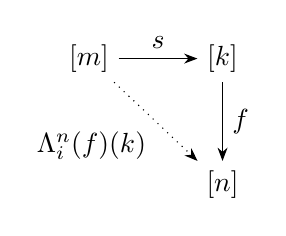
\begin{tikzpicture}[->, >=Stealth]
  % Nodes
	\node (A) {$[m]$};
	\node[right=of A] (B) {$[k]$};
	\node[below=of B] (C) {$[n]$};

  % Arrows (legs of the right triangle)
  \draw (A) -- node[above] {$s$} (B);
  \draw (B) -- node[right] {$f$} (C);

  \draw[dotted] (A) -- node[below left] {$\L^n_i(f) (k)$} (C);
\end{tikzpicture}
$$

$\L^n_i [m]$ is a functor from $\D\op$ to $\S$ by the standard arguments of pullback.
Because $f \in \L^n_i[k]$, $f$ must miss at least one element in $[n] \smallsetminus \{i\}$, so must $f \circ s$.
Therefore the requirement that $\L^n_i(s) (f) \in \L^n_i [m]$ is satisfied, and the definition is self-consistent.

For each $[m]$, $\L^n_i[m]$ is an subset of $\Delta^n[m]$. Moreover, any $f \in \H_{\D}([m], [k])$, $\Delta^n(f)$ restricts to a map from $\L^n_i[k]$ to $\L^n_i[m]$.
Therefore, we may consider $\L^n_i$ as some kind of a sub-simplicial set of $\Delta^n$.

This intuition is further justified by the geometric realisation of $\L^n_i$, denoted as $|\L^n_i|$, which is $|\Delta^n|$ with the interior and the $i$-th face removed. 
See the following figure for horns contained in the $\Delta^2$.

% Demonstration of horns in 2-simplex
$$
\begin{tikzpicture}[scale=1.2, every node/.style={font=\small}]

% ---- 0-simplex ----
\node[circle, fill=black, inner sep=1.5pt] (v0a) at (0,0) {};
\node[circle, fill=black, inner sep=1.5pt] (v0b) at (1.5,0) {};
\node[circle, fill=black, inner sep=1.5pt] (v0c) at (0.75,1.3) {};
\node[below=2pt] at (v0) {$0$};

\draw (v0b) -- (v0a) -- (v0c);

\node[below=2pt] at (v0a) {$0$};
\node[below=2pt] at (v0b) {$1$};
\node[above=2pt] at (v0c) {$2$};

\node[below=12pt] at (0.75,0) {$|\L^2_0|$};

% ---- 1-simplex ----
\node[circle, fill=black, inner sep=1.5pt] (v1a) at (3.5,0) {};
\node[circle, fill=black, inner sep=1.5pt] (v1b) at (5,0) {};
\node[circle, fill=black, inner sep=1.5pt] (v1c) at (4.25,1.3) {};

\draw (v1a) -- (v1b) -- (v1c);

\node[below=2pt] at (v1a) {$0$};
\node[below=2pt] at (v1b) {$1$};
\node[above=2pt] at (v1c) {$2$};

\node[below=12pt] at (4.25,0) {$|\L^2_1|$};

% ---- 2-simplex ----
\node[circle, fill=black, inner sep=1.5pt] (v2a) at (7,0) {};
\node[circle, fill=black, inner sep=1.5pt] (v2b) at (8.5,0) {};
\node[circle, fill=black, inner sep=1.5pt] (v2c) at (7.75,1.3) {};

% \filldraw[fill=gray!20, draw=black] 
\draw (v2a.center) -- (v2c.center) -- (v2b.center);

\node[below=2pt] at (v2a) {$0$};
\node[below=2pt] at (v2b) {$1$};
\node[above=2pt] at (v2c) {$2$};

\node[below=12pt] at (7.75,0) {$|\L^2_2|$};

\end{tikzpicture}
$$

\section{\texorpdfstring{$\infty$}--category via Simplicial Sets}

With the definitions of horns and simplices settled, we are now ready to present one defintion of small $\infty$-categories via simplicial sets.

\subsection{Weak Kan Extension Condition}

\begin{definition}[$\infty$-category]\label{def:infinity-cat}
	An $\infty$-category, $\mathcal{D}$ is a simplicial set that satisfies the inner horn-filling conditions.

	Specifically, for each $n \geq 2$ and $0 < i < n$, any map of from the $i$th horn $f: \L^n_i \to \mathcal{D}$ can be extended to a map $\overline{f}: \Delta^n \to \mathcal{D}$ such that the following diagram commutes:

$$
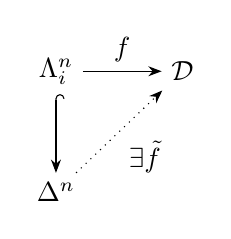
\begin{tikzpicture}[>=Stealth]
  % Nodes
	\node (A) {$\L^n_i$};
	\node[right=of A] (B) {$\mathcal{D}$};
	\node[below=of A] (C) {$\Delta^n$};

  % Arrows (legs of the right triangle)
	\draw[->] (A) -- node[above] {$f$} (B);
	\draw[->, dotted] (C) -- node[below right] {$\exists \tilde{f}$} (B);

  \draw[right hook->] (A) -- node[below left] {} (C);
\end{tikzpicture}
$$

The maps between simplicial sets are natural transformations in $[\D\op, \S]$.
There is no requirement for uniqueness of the extension.

This condition is also known as the \emph{weak Kan extension condition}, and $\infty$-category is also called \emph{weak Kan complex} \cite{boardman2006homotopy}.
\end{definition}

% TODO: is this correct?
In the language of model categories, $\infty$-categories are precisely the fibrant objects in the Joyal model structure on $\sS$ \cite{joyal}.

In this definition, the objects of the $\infty$-category $\mathcal{D}$ are given by the $0$-simplices $\mathcal{D}_0$, the morphisms between two objects $x, y \in \mathcal{D}_0$ are given by the $1$-simplices $f \in \mathcal{D}_1$ such that $d_1(f) = x$ and $d_0(f) = y$. 
Higher objects are given by higher simplices in a similar manner.

An important aspect of this definition is that it allows the composition of morphisms.
For example, given two morphisms $f: x \to y$ and $g: y \to z$ in $\mathcal{D}$, they correspond to two $1$-simplices, and, therefore, a $1$-horn $\L^2_1$ in $\mathcal{D}$.
By the inner horn-filling condition, there exists a $2$-simplex $\sigma \in \mathcal{D}_2$ that fills the horn.
The face map $d^2_1(\sigma)$ then gives a $1$-simplex from $x$ to $z$, which we denote as $g \circ f: x \to z$.
While this composition is not unique, all possible choices of compositions are homotopic via $2$-simplices in $\mathcal{D}$, as we will explain later.

\subsection{Nerves of Categories}

Our first examples of $\infty$-category are the nerves of ordinary categories.

\begin{definition}[Nerves]
	Let $\mathcal{C}$ be an ordinary category.
	Regard $[n]$ as an ordinary category where the objects are elements in $[n]$ and there is a unique morphism from $i$ to $j$ if and only if $i \leq j$.
	The \emph{nerve} of $\C$, denoted as $N(\C)$, is the simplicial set defined as
	\begin{enumerate}
		\item The $n$-simplices are the set of functors from $[n]$ to $\C$, i.e.,
			\begin{equation*}
				N(\C)_n := N(\mathcal{C})([n]) = \F_{\text{Cat}}([n], \mathcal{C}),
			\end{equation*}
		\item The structure maps are induced by the pullbacks along morphisms in $\D$.
			That is for $f \in \H_{\D}([m], [n])$ and $G \in N(\C)([n])$, $N(\C)(f): N(\C)_n \rightarrow N(\C)_m$
			\begin{equation*}
				N(\C)(f) (G) = G \circ f
			\end{equation*}
	\end{enumerate}
\end{definition}

Recall the category $[n]$ is the category induced by the order in the set 
$$\{0 \leq 1 \leq 2 \leq 3 \leq \cdots \leq n\},$$
where a unique morphism exists from $i$ to $j$ if and only if $i \leq j$. 
This is indeed a category, as the identity morphisms of the element $i$ is represented by $i \leq i$, and any compositions of morphisms leads to a unique morphism due to the transitivity of the order relation.

A function from $[n]$ to $\C$ is, therefore, precisely $n+1$ objects in $\C$ with a chain of $n$ morphisms between them, as shown below.
\begin{equation}\label{Nerve-n-chain}
	X_0 \xrightarrow{f_1} X_1 \xrightarrow{f_2} X_2 \xrightarrow{f_3} X_3 \xrightarrow{f_{4}} \cdots \xrightarrow{f_n} X_{n}
\end{equation}
Specifically, $N(\C)_0$ is precisely the objects in $\C$, and $N(\C)_1$ is the collection of morphisms in $\C$.

\begin{remark}\label{nerve-encodes-cat}
	Because $N(\C)_0$ is the objects in $\C$, and $N(\C)_1$ is the morphisms in $\C$, the nerve $N(\C)$ encodes all the data of the ordinary category $\C$. 
\end{remark}

\begin{remark}\label{nerve-face-deg}
Basic chasing of diagrams shows that the face map, $d_i: N(\C)_{n} \rightarrow N(\C)_{n-1}$ sends $n$-chain in \ref{Nerve-n-chain} to $(n-1)$-chain in the following way:
\begin{enumerate}
	\item if $i = 0$, it removes the first object and the first morphism, i.e., \ref{Nerve-n-chain} is sent to
		\begin{equation}
			X_1 \xrightarrow{f_2} X_2 \xrightarrow{f_3} X_3 \xrightarrow{f_{4}} \cdots \xrightarrow{f_n} X_{n}
		\end{equation}
	\item if $0 < i < n$, it removes the $i$-th object and composes the $(i-1)$-th and $i$-th morphisms, i.e., \ref{Nerve-n-chain} is sent to
		\begin{equation}
			X_0 \xrightarrow{f_1} \cdots \xrightarrow{f_{i-1}} X_{i-1} \xrightarrow{f_{i+1} \circ f_i} X_{i+1} \xrightarrow{f_{i+2}} \cdots \xrightarrow{f_n} X_{n}
		\end{equation}
	\item if $i = n$, it removes the last object and the last morphism, i.e., \ref{Nerve-n-chain} is sent to
		\begin{equation}
			X_0 \xrightarrow{f_1} X_1 \xrightarrow{f_2} X_2 \xrightarrow{f_3} \cdots \xrightarrow{f_{n-1}} X_{n-1}
		\end{equation}
\end{enumerate}

Similarly, the degenerate map $s_i: N(\C)_n \to N(\C)_{n+1}$ sends the $n$-chain in \ref{Nerve-n-chain} to the $(n+1)$-chain
\begin{equation}
	X_0 \xrightarrow{f_1} \cdots \xrightarrow{f_{i}} X_{i} \xrightarrow{\text{id}_{X_i}} X_i \xrightarrow{f_{i+1}} \cdots \xrightarrow{f_n} X_{n}
\end{equation}
\end{remark}

The nerves by construction are simplicial sets. An important property is that they are also $\infty$-categories, as stated in the following theorem.

\begin{theorem}
	Let $\C$ be an ordinary category.
	Its nerve $N(\C)$ satisfies the inner horn-filling conditions; therefore is an $\infty$-category.
	Moreover, the extension $\overline{f}: \Delta^n \to N(\C)$ of the map $f: \L^n_i \to N(\C)$ is unique.
\end{theorem}

$$
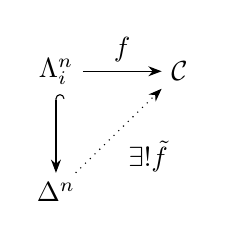
\begin{tikzpicture}[>=Stealth]
  % Nodes
	\node (A) {$\L^n_i$};
	\node[right=of A] (B) {$\C$};
	\node[below=of A] (C) {$\Delta^n$};

  % Arrows (legs of the right triangle)
	\draw[->] (A) -- node[above] {$f$} (B);
	\draw[->, dotted] (C) -- node[below right] {$\exists ! \tilde{f}$} (B);

  \draw[right hook->] (A) -- node[below left] {} (C);
\end{tikzpicture}
$$

\begin{proof}
	Because inner horns are $\L^i_n$ such that $0 < i < n$, we only need to consider the cases for $n \geq 2$.

	Notice $\L^i_n$ has $n$ vertices (the set of vertices is $\L^i_n[0]$). Lable these vertices as $X_0, X_1, \cdots, X_n$.
	Given $f$, we want to find a natural transformations $\tilde{f}\in [\D\op, \S]$, that is, a class of maps $\alpha_{[n]}: \Delta^n \rightarrow N(\C)_n$.

	Notice $\alpha_{[0]}$, a set of $n$ vertices, is completely determined by $f$, so is any $\alpha_{[k]}$ for $k < n - 1$, as $\L^i_n$ only misses one $(n-1)$-simplex, which is the $i$th face, and the only $n$-simplex.
	Therefore, we have the $n$-chain of objects and morphisms in $\C$:
	\begin{equation*}
		X_0 \xrightarrow{f_1} X_1 \xrightarrow{f_2} X_2 \xrightarrow{f_3} X_3 \xrightarrow{f_{4}} \cdots \xrightarrow{f_n} X_{n}
	\end{equation*}
	Where $X_j = \alpha_{[0]}(j)$ and $f_j$ is the morphism from $X_{j-1}$ to $X_j$ induced by $\alpha_{[1]}$. 
	The existence of $f_i$ is clear for $n \geq 3$. 
	For $n = 2$, the only inner horn is $\L^2_1$, which contains the morphisms from $X_0$ to $X_1$ and from $X_1$ to $X_2$, so $f_1$ and $f_2$ are also well-defined.

	This is precisely $\alpha_{[n]}[n]$ we are looking for.
	And the missing $i$-th face is given by the face map $d_i$ applied to this $n$-chain.

\end{proof}



\newpage
\printbibliography[heading=bibintoc]

\end{document}
